\section*{Introducció}

Aquest projecte té com a objectiu dissenyar i implementar una eina d'anàlisi estàtica de software mitjançant grafs de dependències i fluxos d'execució.

\section*{Contextualització}
\subsection*{Anàlisi estàtica de software}
L'anàlisi estàtica de software és una tècnica que consisteix a examinar el codi font d'un programa sense executar-lo. Aquesta tècnica té l'objectiu d'identificar errors, vulnerabilitats i altres problemes relacionats amb el codi \cite{static_code_analysis_jetbrains}. A més, permet analitzar les dependències entre els diferents components del programa i els fluxos d'execució, ajudant a identificar altres possibles problemes. Un altre avantatge d'aquesta anàlisi és que, en cas d'haver de modificar alguna part del codi, permet identificar quines altres parts poden veure's afectades.


\subsection*{Representació del codi i arbres sintàctics}
L'anàlisi estàtica de software no treballa habitualment directament sobre el codi font, sinó sobre una representació estructurada d'aquest. Una de les representacions més habituals és l'AST (Abstract Syntax Tree), un arbre que representa l'estructura sintàctica del programa i les relacions entre els seus diferents elements. Tanmateix, l'AST no conté tota la informació necessària per analitzar el comportament del programa, ja que el seu objectiu principal és representar-ne l'estructura sintàctica. Per exemple, l'ordre i les possibles rutes d'execució del programa requereixen altres representacions, com els grafs de flux d'execució.

Per obtenir l'AST, el codi font passa per diferents fases d'anàlisi. Inicialment, l'anàlisi lèxica divideix el codi en tokens, identificant i classificant les diferents unitats lèxiques que el formen. Aquest procés es podria comparar amb agafar una frase i identificar la categoria de cadascuna de les seves paraules. Posteriorment, l'anàlisi sintàctica utilitza aquests tokens per comprovar si compleixen les regles gramaticals del llenguatge i construir una representació de la seva estructura, com l'AST. Seguint amb l'analogia lingüística, aquesta fase seria equivalent a comprovar si les paraules d'una frase estan ordenades d'acord amb les regles gramaticals.

Un cop comprovada l'estructura sintàctica, es pot realitzar l'anàlisi se\-màntica, que comprova que les construccions del programa tinguin un significat vàlid segons les regles del llenguatge. Per exemple, intentar modificar el valor d'una variable immutable pot ser sintàcticament correcte, però donar lloc a un error semàntic, ja que aquesta operació no és vàlida. De manera similar, en l'analogia lingüística, una frase pot tenir una estructura sintàctica vàlida però contenir combinacions de paraules que no siguin correctes; com podria ser un article femení acompanyant un nom masculí.

A partir d'aquestes representacions i de la informació obtinguda durant les diferents fases d'anàlisi, les eines de processament de codi poden construir estructures que permetin realitzar diferents tipus d'anàlisi estàtica \cite{clang_llvm}\cite{balapriya_ast}.

\subsection*{Grafs de dependències i fluxos d'execució}
En l'àmbit de l'anàlisi estàtica de codi és molt valuós saber no només com s'estructura el codi, sinó també com es relacionen els diferents elements entre sí. Per analitzar aquestes relacions, existeixen els grafs de dependències, a partir dels quals podem observar i analitzar quines afectacions pot tenir una certa modificació en la resta del codi, quines instruccions depenen de les dades produïdes per una instrucció prèvia o, fins i tot, identificar de quina manera es podria paral·lelitzar l'execució del programa \cite{gfg_dependencygraph}.

Una altra representació molt interessant són els grafs de flux d'execució. Aquests grafs tenen una missió molt simple: representar els possibles camins de control que pot seguir l'execució d'un programa. Aquesta informació és molt útil per diverses raons. En primer lloc, permet calcular la complexitat ciclomàtica del programa, que pot utilitzar-se com a indicador de la seva complexitat estructural.

En segon lloc, és útil de cara a testejar el software, ja que permet identificar els diferents camins i condicions de control que poden produir-se durant l'execució. D'aquesta manera, es poden dissenyar proves que cobreixin diferents camins d'execució, incloent-hi casos extrems.

Finalment, de cara a depurar o mantenir el codi, aquesta representació ajuda a acotar la quantitat de camins que s'han d'analitzar. Això pot evitar una pèrdua excessiva de temps a l'hora d'identificar quin camí d'execució està donant problemes o quines parts del codi poden veure's afectades per una modificació \cite{gfg_controlflowgraph}.


\subsection*{Eines i enfocaments existents}


\subsection*{Context i motivació del projecte}
Tot i l'existència d'eines d'anàlisi estàtica, aquestes poden estar orientades a objectius concrets o limitar-se a determinats llenguatges i tipus d'anàlisi. En aquest context, aquest projecte proposa el desenvolupament d'una eina centrada en la representació de les relacions entre els diferents elements del codi mitjançant una abstracció comuna als diferents llenguatges analitzats, permetent posteriorment realitzar diferents tipus d'anàlisi sobre aquesta representació.

A més, es proposa una solució visual i senzilla, amb l'objectiu de facilitar-ne l'ús i permetre una interacció més còmoda per part de l'usuari.

Per últim, aquesta abstracció permet unificar la representació dels diferents elements del codi, deixant oberta la possibilitat d'incorporar l'ús de tècniques d'intel·ligència artificial en un futur.


\section*{Objectius}
\begin{objectius}

\objectiu{
    Dissenyar una eina d'anàlisi estàtica de software.
}{
    Aquesta eina permetrà analitzar i identificar de manera visual les dependències i fluxos d'execució del programa, exposant possibles problemes en el disseny del software.
}

\objectiu{
    Fer l'eina independent del llenguatge de programació analitzat.
}{
    Aquest objectiu permet convertir l'eina en un programa reutilitzable i adaptable a diferents llenguatges de programació, augmentant la seva versatilitat i potencial d'ús.
}

\objectiu{
    Analitzar les dependències entre els diferents components del programa.
}{
    Aquest anàlisi permet identificar el grau d'acoblament del programa, així com dependències circulars/innecessàries, identificant a què pot arribar a afectar una modificació en alguna part del codi.
}

\objectiu{
    Analitzar fluxos d'execució del programa.
}{
    Aquest anàlisi permet identificar possibles problemes de concurrència, així com punts o camins crítics en el flux d'execució del programa, ajudant a trobar possibles bottlenecks i punts de millora en el rendiment del software.
}

\objectiu{
    Garantir el correcte funcionament de l'eina amb un subconjunt
    representatiu dels elements del llenguatge analitzat.
}{
    Aquest objectiu permet delimitar l'abast del projecte i establir
    un conjunt concret de funcionalitats sobre les quals avaluar
    el correcte funcionament de l'eina.
}

\objectiu{
    Validar l'eina amb exemples pràctics i casos d'ús reals.
}{
    Aquest objectiu permet extreure conclusions sobre la utilitat de l'eina en casos d'ús reals, així com identificar possibles millores i funcionalitats a implementar.
}

\objectiu{
    Representar visualment els resultats mitjançant grafs.
}{
    Aquesta representació permetrà als usuaris analitzar i comprendre de manera senzilla els resultats obtinguts per l'eina, així com identificar visualment possibles errors o millores en el software.
}

\objectiu{
    Analitzar la utilitat de l'eina en la millora de la qualitat del software.
}{
    Aquest objectiu permetrà avaluar l'impacte de l'eina tant en la millora de la qualitat del software com en la velocitat d'identificació d'errors i punts de millora, a més de la reducció del temps de desnvolupament i manteniment del mateix.
}

\end{objectius}


\section*{Metodologia}
El desenvolupament del projecte seguirà una metodologia iterativa i incremental. Inicialment, es dissenyarà una arquitectura i les principals funcionalitats de l'eina, que posteriorment seran implementades. Durant aquest procés, s'anirà avaluant el correcte funcionament de les característiques implementades mitjançant proves, a més de les reunions de seguiment periòdiques amb el tutor. En cas de detectar errors o mancances, es revisarà el disseny per tal de corregir-los o incorporar els elements necessaris. L'objectiu principal d'aquesta metodologia és mantenir un desenvolupament àgil i flexible, prioritzant la netedat i la qualitat del software desenvolupat.
En quant als objectius, aquests serviran per marcar les fites del projecte, ja que cada un d'ells comporta un conjunt de fncionalitats a implementar. Es considerarà com a complert un objectiu quan s'hagin implementat i testejat totes les funcionalitats necessàries.

\section*{Planificació}
\begin{figure}[ht]
    \centering
    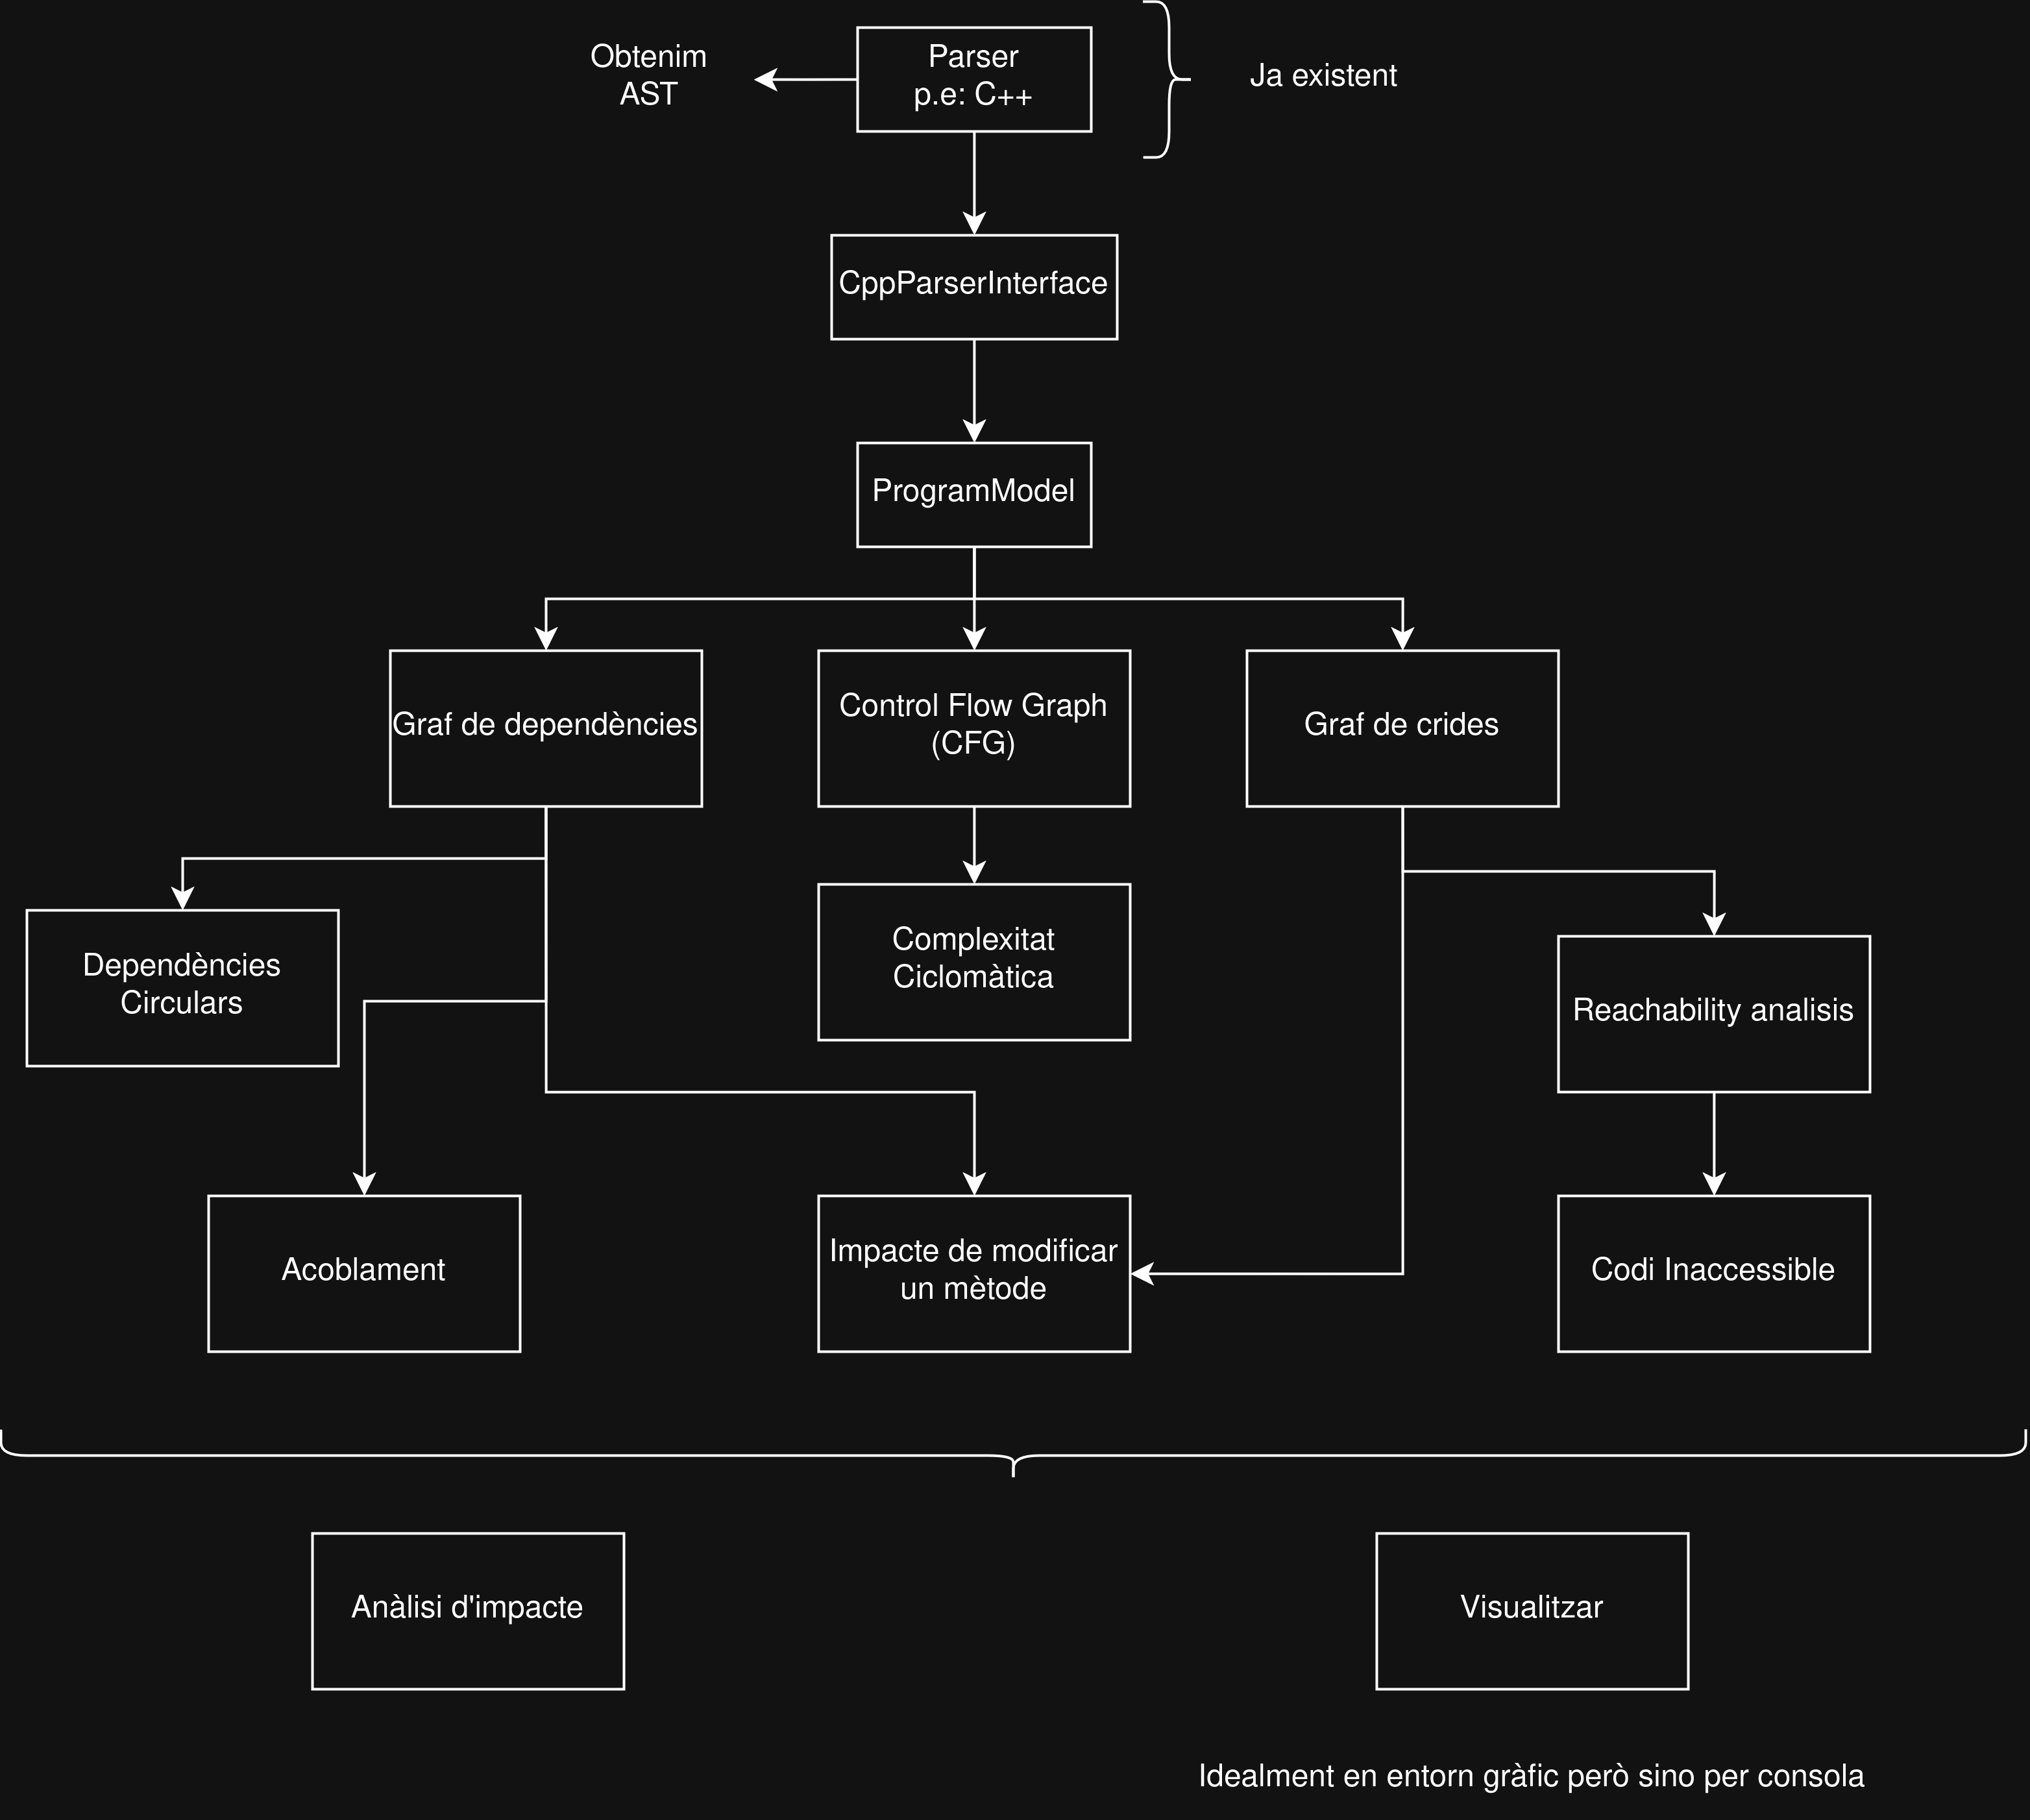
\includegraphics[width=0.8\textwidth]{figures/estructura_inicial_TFG.png}
    \caption{Arquitectura general de l'eina.}
    \label{fig:arquitectura}
\end{figure}

\section*{Ús de la IA}
Durant l'elaboració d'aquest informe inicial, s'ha utilitzat la IA, concretament la versió gratuita de ChatGPT. Ha tingut la funció de millorar la redacció i la gramàtica del text, a més de respondre a consultes sobre com dur a terme determinades coses en LaTeX. A més a més, s'ha utilitzat per a realitzar búsquedes d'informació sobre projectes o papers rellevants.
Quant al desenvolupament del projecte, la IA tindrà un paper similar. A més a més, s'utilitzarà, de forma molt guiada, per a generar fragments de codi però, no per a generar l'arquitectura de l'eina ni per a generar funcionalitats completes. Per tant, la IA tindrà un paper de suport, ajudant a millorar la productivitat i eficiència del treball realitzat però, en cap cas, substituint la feina de l'autor del projecte.

\printbibliography
